\title{Parametric Vector Form} 
\subtitle{\SubTitleName}
\institute[]{\Course}
\author{\Instructor}
\maketitle   


\begin{frame}
\frametitle{Motivating Questions}

     
 
    \begin{center}\begin{tikzpicture} \node [mybox](box){\begin{minipage}{0.95\textwidth} \vspace{2pt}
                \onslide<1->{How can we express the set of solutions to a \textbf{consistent} system \textbf{with free variables} in a concise form?} \onslide<2->{How do we obtain this representation?  }
    \end{minipage}};
    \end{tikzpicture}\end{center}

    \onslide<3->{
    
    \LO\\

    \LearningObjectiveStatement

    \begin{itemize}
        \item express the solution set of a linear equation in parametric vector form
        % \item Provide a geometric interpretation to the solution set of a linear system.
        % \item Characterize homogeneous linear systems using the concepts of free variables, span, pivots, linear combinations, and echelon forms.
    \end{itemize}

    }
\end{frame}

% \frame{\frametitle{Learning Objectives}

%     % \Emph{Topics} \\
%     % \TopicStatement
%     % \begin{itemize}
%     %     % \item homogeneous systems
%     %     \item parametric \Emph{vector} forms of solutions to linear systems
%     % \end{itemize}

%     % \vspace{0.5cm}

%     % \LO\\
    
%     \LearningObjectiveStatement

%     \begin{itemize}
%         \item express the solution set of a linear equation in parametric vector form
%         % \item Provide a geometric interpretation to the solution set of a linear system.
%         % \item Characterize homogeneous linear systems using the concepts of free variables, span, pivots, linear combinations, and echelon forms.
%     \end{itemize}
% }



% \begin{frame}
% \frametitle{Recall: Homogeneous Systems}

%     \begin{center}\begin{tikzpicture} \node [draw,rounded corners,fill=gray!10](box){\begin{minipage}{0.90\textwidth}\vspace{4pt}

%         Linear systems of the form $A\vec x = \vec 0$ are \textbf{homogeneous}. \\[12pt]
%         Linear systems of the form $A\vec x = \vec b, \ \vec b \neq \vec 0$, are \textbf{inhomogeneous}.
        
%     \end{minipage}};
%     \end{tikzpicture}\end{center}    

%     \vspace{12pt}
%     These systems are related to each other in a way that is easier to see with \textbf{parametric vector form}. 

% \end{frame}

\begin{frame}
\frametitle{Example: One Homogeneous Equation in Two Variables}
\vspace{-12pt}

\begin{align*}
    x_1 + 2x_2 &= 0
\end{align*}

\vspace{4pt}

\pause The basic variable is $x_1$, the free variable is $x_2$. \pause The solution set is the line $x_2 = -x_1 / 2$ which passes through the origin.
\pause

    \begin{center}
    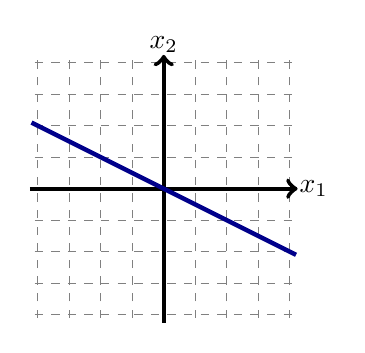
\begin{tikzpicture}[scale=.4]
    \draw[help lines,gray,dashed] (-4.1, -4.1) grid (4.1, 4.1);
    \draw[ultra thick, ->] (-4.25, 0) -- (4.25, 0);
    \draw[ultra thick, ->] (0, -4.25) -- (0, 4.25);
    \node[above] at (0, 4) {$x_2$};
    \node[right] at (4, 0) {$x_1$};
    \pause
        \draw[ultra thick, -, DarkBlue] (-4.2, 2.1) -- (4.2,-2.1);
    \end{tikzpicture}
    \end{center}

\end{frame}

\begin{frame}
\frametitle{Example: Obtaining Parametric Vector Form}
How can we express the solution set in more complex situations? \onslide<2->{ Express basic variables in terms of free variables:}
\begin{align*}
    \onslide<3->{x_1+ 2x_2 = 0 \onslide<4->{\quad \Rightarrow \quad x_1 = -2x_2}}
\end{align*}
\onslide<5->{Now we can express the solution as:}
\begin{align*}
    \onslide<5->{
    \vec{x} = \begin{pmatrix} x_1 \\ x_2 \end{pmatrix} = }\onslide<6->{\begin{pmatrix} -2x_2 \\ x_2 \end{pmatrix} = }\onslide<7->{x_2 \begin{pmatrix} -2 \\ 1 \end{pmatrix} = }\onslide<8->{x_2 \vec v, \quad \text{where} \quad \vec v = \begin{pmatrix} -2 \\ 1 \end{pmatrix}}
\end{align*}
    \begin{center}
    \onslide<9->{
    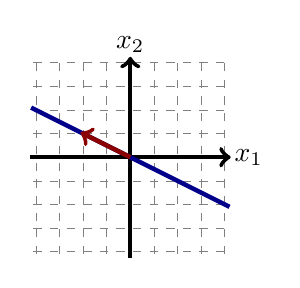
\begin{tikzpicture}[scale=.3 ]
    \draw[help lines,gray,dashed] (-4.1, -4.1) grid (4.1, 4.1);
    \draw[ultra thick, ->] (-4.25, 0) -- (4.25, 0);
    \draw[ultra thick, ->] (0, -4.25) -- (0, 4.25);
    \node[above] at (0, 4) {$x_2$};
    \node[right] at (4, 0) {$x_1$};
    \draw[ultra thick, -, DarkBlue] (-4.2, 2.1) -- (4.2,-2.1);
    \onslide<10->{\draw[ultra thick, ->, DarkRed] (0,0) -- (-2.1, 1.05);}
    \end{tikzpicture}
    }
    \end{center}
\end{frame}

\begin{frame}
\frametitle{Parametric Vector Form}
The parametric vector form for
$$x_1 + 2x_2 = 0$$
\onslide<2->{is}
\begin{align*}
    \onslide<2->{
    \vec{x} = }\onslide<3->{x_2 \vec v, \quad \text{where} \quad \vec v = \begin{pmatrix} -2 \\ 1 \end{pmatrix}}
\end{align*}

\onslide<4->{The solution set: consists of all scalar multiples of a single vector.}

\onslide<5->{Procedure for obtaining parametric vector form: }

\begin{enumerate}
    \item<6-> Reduce system to RREF.
    \item<7-> Express basic variables in terms of free variables.
    \item<8-> Substitute expressions into $\vec x$.
    \item<9-> Express solution vector $\vec x$ in terms of a set of vectors and parameters.
\end{enumerate}

\end{frame}

\begin{frame}
\frametitle{Exercise}
What is the parametric vector form for the equation? 
$$3x_1 - 12x_2 = 0$$

\end{frame}

\begin{frame}
\frametitle{Summary: Parametric Vector Form}
For a single equation in two variables:
\begin{itemize}
    \item<2-> \textbf{Solution set:} consists of all scalar multiples of a single vector.
    \item<3-> \textbf{Parametric vector form: } expresses the solution set in terms of a parameter, $x_2$, and a vector, $\vec v$.
    \item<4-> \textbf{Procedure for obtaining parametric vector form: } 1) reduce system to RREF, 2) express basic variables in terms of free variables, 3) substitute into $\vec x$, 4) express solution in terms of a set of vectors and parameters.
    \item<5-> \textbf{Next: }how can we apply this representation to larger systems?  
\end{itemize}

\end{frame}

% \begin{frame}
% \frametitle{Example 2: Homogeneous System in $\mathbb{R}^3$ (Setup)}
% Consider the system:
% \begin{align*}
%     x_1 + x_2 &= 0 \\
%     x_2 + x_3 &= 0
% \end{align*}
% \pause
% Expressing as an augmented matrix and row reducing:
% \begin{align*}
%     \begin{amatrix}{3}
%         1 & 1& 0 & 0 \\ 0&1&1&0
%     \end{amatrix}
%     = 
%     \begin{pmatrix} 1 & 1 & 0 \\\ 0 & 1 & 1 \end{pmatrix} 
%     &\sim \begin{pmatrix} 1 & 1 & 0 \\\ 0 & 1 & 1 \end{pmatrix}
% \end{align*}
% \end{frame}

% \begin{frame}
% \frametitle{Example 2: Solving for Basic Variables}
% Solving for the basic variables:
% \begin{align*}
%     x_1 &= -x_2 \\
%     x_3 &= -x_2
% \end{align*}
% \pause
% Expressing in parametric vector form:
% \begin{align*}
%     \vec{x} = x_2 \begin{pmatrix} -1 \\ 1 \\ -1 \end{pmatrix}
% \end{align*}
% \end{frame}


% \begin{frame}
% \frametitle{Example 2: Interpretation of the Solution}
% \textbf{Analysis:} The solution set consists of all linear combinations of the two direction vectors. Since there are two free variables, the solution set forms a line through the origin in $\mathbb{R}^3$.
% \end{frame}

% \begin{frame}
% \frametitle{Example 3: Inhomogeneous System (Setup)}
% Consider the system:
% \begin{align*}
%     x_1 + x_2 &= 3 \\
%     x_2 + x_3 &= 1
% \end{align*}
% \pause
% Expressing as an augmented matrix and row reducing:
% \begin{align*}
%     \begin{pmatrix} 1 & 1 & 0 & \bigm| 3 \\\ 0 & 1 & 1 & \bigm| 1 \end{pmatrix} 
%     &\sim \begin{pmatrix} 1 & 1 & 0 & \bigm| 3 \\\ 0 & 1 & 1 & \bigm| 1 \end{pmatrix}
% \end{align*}
% \end{frame}

% \begin{frame}
% \frametitle{Example 3: Solving for Basic Variables}
% Solving for the basic variables:
% \begin{align*}
%     x_1 &= 3 - x_2 \\
%     x_3 &= 1 - x_2
% \end{align*}
% \pause
% Expressing in parametric vector form:
% \begin{align*}
%     \vec{x} = \begin{pmatrix} 3 \\ 0 \\ 1 \end{pmatrix} + x_2 \begin{pmatrix} -1 \\ 1 \\ -1 \end{pmatrix}
% \end{align*}
% \end{frame}

% \begin{frame}
% \frametitle{Example 3: Interpretation of the Solution}
% \textbf{Analysis:} Unlike the previous homogeneous cases, the solution set is not a subspace. Instead, it is a translated version of the homogeneous solution set, shifted by the vector $\begin{pmatrix} 3 \\ 0 \\ 1 \end{pmatrix}$. This means the solution set forms a line that does not pass through the origin.
% \end{frame}


% \begin{frame}
% \frametitle{Recall: Homogeneous Systems}

%     \begin{center}\begin{tikzpicture} \node [mybox](box){\begin{minipage}{0.90\textwidth}\vspace{4pt}

%         Linear systems of the form $A\vec x = \vec 0$ are \Emph{homogeneous}. \\[12pt]
%         Linear systems of the form $A\vec x = \vec b, \ \vec b \ne \vec 0$, are \Emph{inhomogeneous}.
        
%     \end{minipage}};
%     \node[fancytitle, right=10pt] at (box.north west) {Definition};
%     \end{tikzpicture}\end{center}    

%     \vspace{12pt}
    
%     These systems are related to each other in a way that is easier to see with \Emph{parametric vector form}. 

% \end{frame}


% \begin{frame}
% \frametitle{Parametric Vector Form for the Non-homogeneous Case}
%     Write the solution as a sum of vectors. 
%     \pause
%     \begin{align*}
%         2x_1 + x_2 &= 4 \\
%         4x_1 + 2x_2 &= 8
%     \end{align*}
% \end{frame}

% \begin{frame}
% \frametitle{Row Reduce}
%     Expressing the system as an augmented matrix and row reducing yields:\pause 
%     \begin{align*}
%         \begin{pmatrix} 2&1&4\\4&2&8\end{pmatrix} 
%         &\sim \begin{pmatrix} 2&1&4\\0&0&0\end{pmatrix}, \ R_2 - 2R_1 \to R_2
%     \end{align*}
%     \pause 
%     This gives us one equation: $2x_1 + x_2 = 4$. \pause
    
%     Therefore $x_2$ is free, and $x_1 = 2 - \frac{1}{2}x_2$.
%     Expressing as a vector equation: 
%     $$\begin{pmatrix} \vec x = \begin{pmatrix} x_1 \\ x_2 \end{pmatrix}\end{pmatrix} = \begin{pmatrix} 2-x_2/2 \\x_2 \end{pmatrix}$$
% \end{frame}

% \begin{frame}
% \frametitle{Parametric Vector Form}
%     \onslide<2->{We found that $x_2$ is free and $x_1 = 2 - \frac{1}{2}x_2$} 
%     \onslide<3->{Our goal is to now express the solution set as a sum of vectors.} 
%     \onslide<4->{Note that solutions to the system will be vectors in $\mathbb R^2$. So if $\vec x$ is a solution, then}
%     $$\onslide<5->{ \vec x = \begin{pmatrix} x_1\\x_2\end{pmatrix}}$$
% \end{frame}


% \begin{frame}
% \frametitle{Parametric Vector Form for the Non-homogeneous Case}

%     Write the solution as a sum of vectors. In other words, express the solution in parametric vector form. Give a geometric interpretation of the solution.
%     \begin{align*}
%         x_1 + 3x_2 + x_3 &=4 \\
%         2x_1 -x_2 - 5x_3 &= 1 \\
%         x_1 - 2x_3 &=1
%     \end{align*}

%     \textit{Note that the left-hand side is the same as a previous example}.  

% \end{frame}


% \begin{frame}
% \frametitle{Row Reduce}

%     Expressing the system as an augmented matrix and row reducing yields:
%     \begin{align*}
%         \begin{pmatrix} 1&3&1&4\\2&-1&-5&1\\1&0&-2&1\end{pmatrix} 
%         &\sim \begin{pmatrix} 1&3&1&4\\0&-7&-7&-7\\1&0&-2&1\end{pmatrix}, \ R_2 - 2R_1 \to R_2 \\
%         &\sim \begin{pmatrix} 1&3&1&4\\0&1&1&1\\0&-3&-3&-3\end{pmatrix} \\
%         &\sim \begin{pmatrix} 1&0&-2&1\\0&1&1&1\\0&0&0&0\end{pmatrix} 
%     \end{align*}
%     Therefore $x_3$ and $x_4$ are free, $x_1 = 2x_3-x_4$, and $x_2 = -x_3-x_4$.

% \end{frame}


% \begin{frame}
% \frametitle{Parametric Vector Form}

%     \onslide<2->{We found that $x_3$ and $x_4$ are free, $x_1 = 2x_3-x_4$, and $x_2 = -x_3-x_4$} \onslide<3->{Our goal is to now express the solution set as a sum of vectors. } \onslide<4->{Note that solutions to the system will be vectors in $\mathbb R^4$. So if $\vec x$ is a solution, then}
%     $$\onslide<5->{\vec x = \begin{pmatrix} x_1\\x_2\\x_3\\x_4\end{pmatrix}}$$

% \end{frame}





% \begin{frame}\frametitle{Parametric Forms, Homogeneous Case}

%     In general, suppose the free variables for $A \vec x= \vec 0$ are $x_k,\ldots,x_n$. Then all solutions to $A \vec x= \vec 0$ can be written as
%     \begin{align*}
%         \vec x = x_k \vec v_k + x_{k+1} \vec v_{k+1}+\cdots + x_n \vec v_n
%     \end{align*}
%     for some $\vec v_k,\ldots,\vec v_n$. This is the \Emph{parametric form} of the solution.

% \end{frame}

% \frame{\frametitle{Summary}

% \SummaryLine \vspace{4pt}
% \begin{itemize}\setlength{\itemsep}{8pt}
%     \item expressing the solution set of a linear system in parametric vector form
%     \item the geometric relationship between the solution to $A\vec x = \vec b$ and $A\vec x = \vec 0$
% \end{itemize}

% }




%\begin{frame}
%Then, you add to this (or any other) particular solution the parametric form of your homogeneous solution: 
%\begin{equation*}
%\begin{bmatrix*}[r]
%1 & 1 & -3 \\ 1 & -1 & 1 \\ -1 & 5 & -7 
%\end{bmatrix*}
%\begin{bmatrix*}[r]
%2 \\ 5 \\ 3
%\end{bmatrix*} = \vec 0 
%\end{equation*}
%And the matrix only has one free variable, call it $ x_3$, so our parameterized solution to the non-homogeneous solution is 
%\begin{equation*}
%\begin{bmatrix*}[r]
%-1 \\- 1 \\ 1  
%\end{bmatrix*} + x_3 \begin{bmatrix*}[r]
%2 \\ 5 \\ 3
%\end{bmatrix*} 
%\end{equation*}
%\end{frame}
